%----------------------------------------------------------------------------------------
%	PACKAGES AND DOCUMENT CONFIGURATIONS
%----------------------------------------------------------------------------------------

\documentclass{article}


\usepackage{graphicx} % Required for the inclusion of images
\usepackage{subfigure} % Required for the inclusion of images
\usepackage{natbib} % Required to change bibliography style to APA
\usepackage{amsmath} % Required for some math elements
\usepackage{float}

\usepackage{xcolor}
\usepackage{listings}
\lstset{
    basicstyle=\footnotesize \ttfamily ,
	escapeinside=``,
	linewidth=\textwidth,
	numbers=left,
	numberstyle=\footnotesize  \ttfamily \color{blue},
	frame=trbl,
	aboveskip=1em,
	framextopmargin=2pt,framexbottommargin=2pt,abovecaptionskip=-3pt,belowcaptionskip=3pt,
} %Required for inserting code

%\usepackage{times} % Uncomment to use the Times New Roman font

%----------------------------------------------------------------------------------------
%	DOCUMENT INFORMATION
%----------------------------------------------------------------------------------------

\title{\textbf{Project 1: Optimizing the Performance of a Pipelined Processor}} % Title

\author{519030910210, Wanting Li, liwanting\_2001@sjtu.edu.cn\\
		519021911045, Weihao Jiang, weihao.jiang@sjtu.edu.cn}% Author name and email

\date{\today} % Date for the report

\setlength{\parindent}{0pt}
\setlength{\parskip}{1ex}
\begin{document}

\maketitle % Insert the title, author and date

\section{Introduction}

In this project, we experimentally learn about the design and implementation of a pipelined Y86 processor step by step. Firstly, we write three simple assembly programs to implement three functions in \texttt{example.c} in part A. And in part B, we implement new instruction \texttt{iaddl} and modify the \texttt{HCL} file of the Y86's sequential design. Finally, we optimize the Y86 benchmark program and the processor design with the achievement of the previous two part in part C.

After completing this project, we become more familiar with linux operations and computer architecture and have a keen insight into the interactions between code and hardware that affect the performance of programs.

\textbf{Contribution}
	\begin{itemize}
		\item \textbf{Weihao Jiang}: Code of Part A(\texttt{rsum.ys} and \texttt{copy.ys}) and Part C, Report of Part C
		\item \textbf{Wanting Li}: Code of Part A(\texttt{sum.ys}) and Part B, Report of Remaining Parts
	\end{itemize}
\section{Experiments}

\subsection{Part A}

\subsubsection{Analysis}

In this part, we write and simulate three Y86 programs, whose behavior is defined by the functions in \texttt{example.c}. It is quite trivial to reach the basic requirements. However, how to optimize to achieve a  better performance and code elegance is worth exploring.

\begin{itemize}
	\item \textbf{Difficult Point}
		\begin{itemize}
			\item Prevent from covering the values of registers by mistake.
			\item Be careful to the order of pulling elements from stack.
			\item Be careful to implement the function recursion.
		\end{itemize}
	\item \textbf{Core Technique}
		\begin{itemize}
			\item Divide every function into several smaller parts according to its semantic.
			\item Draw a picture of stack to update the status of stack and ensure the correctness of fetching variables.
		\end{itemize}
\end{itemize}
\subsubsection{Code}

\begin{itemize}
	\item \textbf{sum.ys}

\begin{lstlisting}
# Weihao Jiang: 519021911045
# Wanting Li: 519030910210

# Execution begins at address 0
	.pos	0
init:
	irmovl	Stack,	%esp	# Set up stack pointer
	rrmovl	%esp,	%ebp	# Set up base pointer
	irmovl	ele1,	%eax
	pushl	%eax
	call	Main		# Execute main program
	halt			# Terminate program

# Sample linked list
	.align	4
ele1:
	.long	0x00a
	.long	ele2
ele2:
	.long	0x0b0
	.long	ele3
ele3:
	.long	0xc00
	.long	0

# int sum_list(list_ptr ls)
Main:
	pushl 	%ebp		# save a copy of Main's ebp
	rrmovl 	%esp ,	%ebp	# initialize frame
	xorl 	%eax ,	%eax	# clear eax
	mrmovl	8(%ebp),%edx	# edx = ls
	andl	%edx,	%edx	# ls ?= 0
	je	End		# if(ls == 0) goto End
Loop:
	mrmovl	(%edx),	%ecx	# tmp = ls->val
	addl	%ecx ,	%eax	# val += tmp
	mrmovl	4(%edx),%edx	# ls = ls->next
	andl	%edx,	%edx
	jne	Loop		# if edx == 0 break
End:
	rrmovl 	%ebp ,	%esp	# resume esp and ebp of Main
	popl 	%ebp
	ret

# Stack
	.pos 0x100
Stack:

\end{lstlisting}
\vspace{6ex}
	\item \textbf{rsum.ys}

\begin{lstlisting}
# Weihao Jiang: 519021911045
# Wanting Li: 519030910210

# Execution begins at address 0
	.pos 0
init:	irmovl Stack, %esp  	# Set up stack pointer
	irmovl Stack, %ebp  	# Set up base pointer
	call Main		# Execute main program
	halt			# Terminate program

# Sample linked list
    .align 4
ele1:
    .long 0x00a
    .long ele2
ele2:
    .long 0x0b0
    .long ele3
ele3:
    .long 0xc00
    .long 0

Main:	pushl	%ebp
	rrmovl	%esp,%ebp
	irmovl	ele1,%edx
	pushl	%edx		# Push linklist head
	call	sum		# rsum_list(ele1)

	rrmovl	%ebp,%esp
	popl	%ebp
	ret

# int rsum_list(list_ptr ls)
sum:	pushl	%ebp
	rrmovl	%esp,%ebp

	mrmovl	8(%ebp),%edx    # edx = ls
	andl	%edx,%edx
	je	Nullptr         # if (!ls)

	mrmovl	4(%edx),%ecx    # ecx = ls->next
	pushl	%ecx            # rsum_list(ecx)
	call	sum
	mrmovl	8(%ebp),%edx    # edx = ls
	mrmovl	0(%edx),%ebx    # ebx = ls->val
	addl	%ebx, %eax      # eax += ebx

	rrmovl	%ebp,%esp
	popl	%ebp
	ret
Nullptr:
	xorl	%eax,%eax	#  return 0;
	rrmovl	%ebp,%esp
	popl	%ebp
	ret

# The stack starts here and grows to lower addresses
	.pos 0x100
Stack:

\end{lstlisting}
\vspace{6ex}
	\item \textbf{copy.ys}

\begin{lstlisting}
# Weihao Jiang: 519021911045
# Wanting Li: 519030910210

# Execution begins at address 0
	.pos 0
init:
	irmovl Stack, %esp
	irmovl Stack, %ebp
	call Main
	halt

# Sample structure
	.align 4
list:
	.long 0x00a
	.long 0x0b0
	.long 0xc00

Main:
	pushl	%ebp
	rrmovl	%esp, %ebp
	irmovl	list, %edx
	pushl	%edx
	irmovl	dest, %edx
	pushl	%edx
	irmovl	$3, %edx
	pushl	%edx
	call	copy		# copy (list, dest, 3)
	rrmovl	%ebp, %esp
	popl	%ebp
	ret

copy:
	pushl	%ebp
	rrmovl	%esp, %ebp
	xorl	%eax,%eax	# result = eax = 0
	mrmovl	8(%ebp),%edx	# edx = 3
	mrmovl	12(%ebp), %ecx	# ecx = dest
	mrmovl	16(%ebp), %ebx	# ebx = list
	pushl	%eax		# push result
	pushl	%edx		# push len
	jmp	whileend	# start while loop

whilestart:
	popl	%eax
	pushl	%edx		# Swap eax and edx in stack
	pushl	%eax
	mrmovl	0(%ebx), %eax	# eax = list
	rmmovl	%eax, 0(%ecx)	# dest = eax
	irmovl	$4, %edx
	addl	%edx, %ebx	# list += 4
	addl	%edx, %ecx	# dest += 4
	popl	%edx		# edx = result
	xorl	%edx, %eax	# eax = result ^ eax
	popl	%edx
	pushl	%eax
	irmovl	$-1, %eax	# swap eax and edx in stack
	addl	%eax, %edx	# len --
	pushl	%edx		# push len and result

whileend:
	popl	%edx
	xorl	%eax, %eax
	subl	%edx, %eax
	jl	whilestart

	popl	%eax
	rrmovl	%ebp, %esp
	popl	%ebp
	ret

	.pos 0x200
Stack:

	.pos 0x300
dest:
\end{lstlisting}

\end{itemize}
\newpage
\subsubsection{Evaluation}

	\begin{itemize}
		\item \textbf{sum.ys}

    \begin{figure}[H]
	\centering
	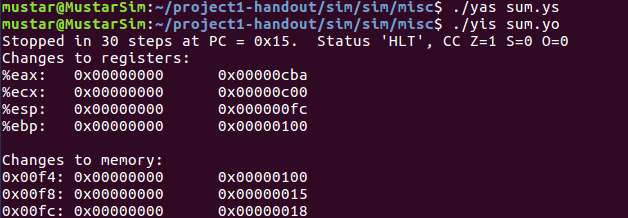
\includegraphics[width=0.9\textwidth]{sum.ys}
	\caption{The result of sum.ys}
	\end{figure}

		\item \textbf{rsum.ys}

    \begin{figure}[H]
	\centering
	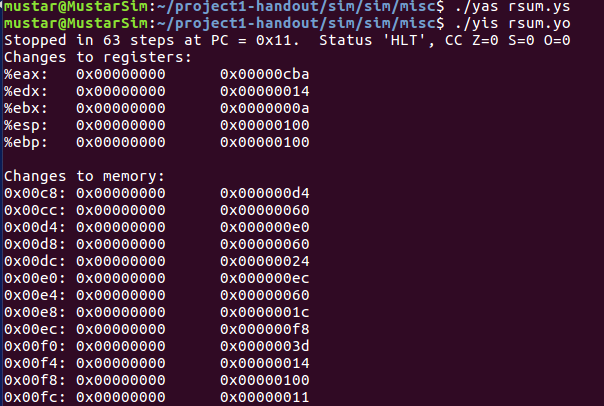
\includegraphics[width=0.9\textwidth]{rsum.ys}
	\caption{The result of rsum.ys}
	\end{figure}
    \newpage
		\item \textbf{copy.ys}

    \begin{figure}[H]
	\centering
	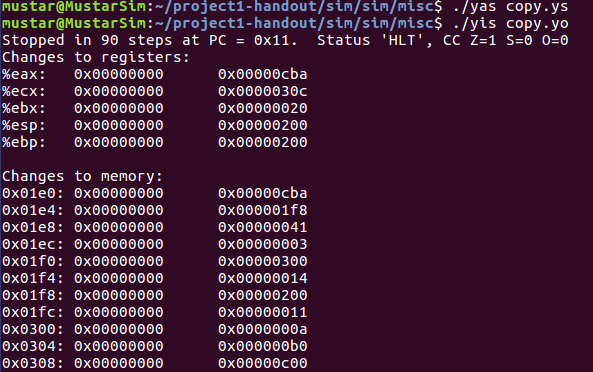
\includegraphics[width=10.5cm]{copy.ys}
	\caption{The result of copy.ys}
	\end{figure}

	\end{itemize}

\subsection{Part B}

\subsubsection{Analysis}

To extend the SEQ processor to support a new instruction \texttt{iaddl}, we could take a look at the processing logic first.
\begin{enumerate}
	\item Get the icode and ifun which combine a byte by M1[PC]
	\item According to the binary code of \texttt{iaddl}, the lower four bits of M1[PC+1] are used, so the register rB is used to add with the constant value. Moreover, the higher four bits of M1[PC+1] is F, so the register rA is not valid. Then, we get the rest lower 4 bytes of the instruction to get the instant
value.
	\item Get the value in the register and store it in valB when decoding the instruction.
	\item Execute the add operation.
	\item Write the result back and update PC to prepare for the next instruction.
\end{enumerate}
Then we can modify \texttt{seq-full.hcl}. And the only difficult point is to understand the syntax of \texttt{HCL}.
\subsubsection{Code}

\begin{lstlisting}
# iaddl:
# Fetch:	icode:ifun	<- M1[PC]
#		rA:rB		<- M1[PC + 1]
#		valC		<- M4[PC + 2]
#		valP		<- PC + 6
# Decode:	valB		<- R[rB]
# Execute:	valE		<- valB + valC
#		Set CC
# Memory:
# Write Back:	R[rB]		<- valE
# PC update:	PC		<- valP

bool instr_valid = icode in
	{ INOP, IHALT, IRRMOVL, IIRMOVL, IRMMOVL, IMRMOVL,
	       IOPL, IJXX, ICALL, IRET, IPUSHL, IPOPL, IIADDL};

# Does fetched instruction require a regid byte?
bool need_regids =
	icode in { IRRMOVL, IOPL, IPUSHL, IPOPL,
		     IIRMOVL, IRMMOVL, IMRMOVL, IIADDL };

# Does fetched instruction require a constant word?
bool need_valC =
	icode in {IIRMOVL,IRMMOVL,IMRMOVL,IJXX,ICALL,IIADDL};

## What register should be used as the B source?
int srcB = [
	icode in { IOPL, IRMMOVL, IMRMOVL, IIADDL  } : rB;
	icode in { IPUSHL, IPOPL, ICALL, IRET } : RESP;
	1 : RNONE;  # Don't need register
];

## What register should be used as the E destination?
int dstE = [
	icode in { IRRMOVL } && Cnd : rB;
	icode in { IIRMOVL, IOPL, IIADDL } : rB;
	icode in { IPUSHL, IPOPL, ICALL, IRET } : RESP;
	1 : RNONE;  # Don't write any register
];

## Select input A to ALU
int aluA = [
	icode in { IRRMOVL, IOPL } : valA;
	icode in { IIRMOVL, IRMMOVL, IMRMOVL, IIADDL } : valC;
	icode in { ICALL, IPUSHL } : -4;
	icode in { IRET, IPOPL } : 4;

## Select input B to ALU
int aluB = [
	icode in { IRMMOVL, IMRMOVL, IOPL, ICALL,
		      IPUSHL, IRET, IPOPL, IIADDL } : valB;
	icode in { IRRMOVL, IIRMOVL } : 0;
	# Other instructions don't need ALU
];

## Set the ALU function
int alufun = [
	icode == IOPL : ifun;
	icode == IIADDL : ALUADD;
	1 : ALUADD;
];

## Should the condition codes be updated?
bool set_cc = icode in { IOPL, IIADDL };
\end{lstlisting}

\subsubsection{Evaluation}

    \begin{figure}[H]
	\centering
	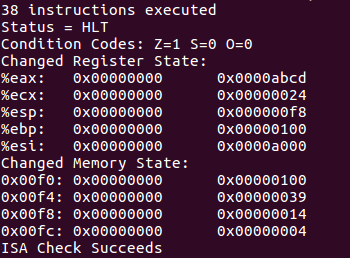
\includegraphics[width=0.6\textwidth]{testing on y86 program}
	\caption{Test \texttt{iaddl} on a simple Y86 program}
	\end{figure}

	\begin{figure}[H]
		\centering
		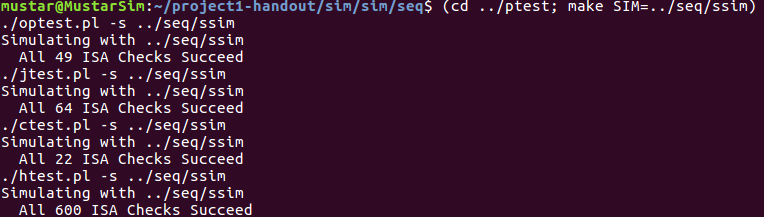
\includegraphics[width=\textwidth]{regression test}
		\caption{Regression test(everything except \texttt{iaddl})}
		\end{figure}

    \begin{figure}[H]
	\centering
	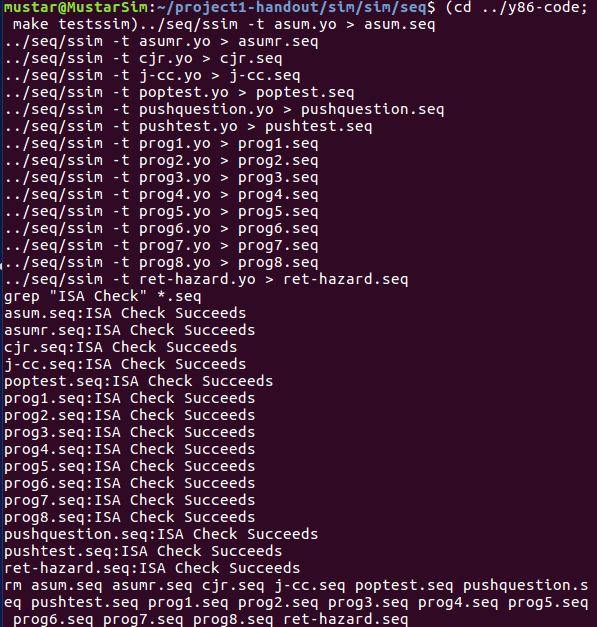
\includegraphics[width=0.7\textwidth]{benchmark retest}
	\caption{Benchmark retest}
	\end{figure}

    \begin{figure}[H]
	\centering
	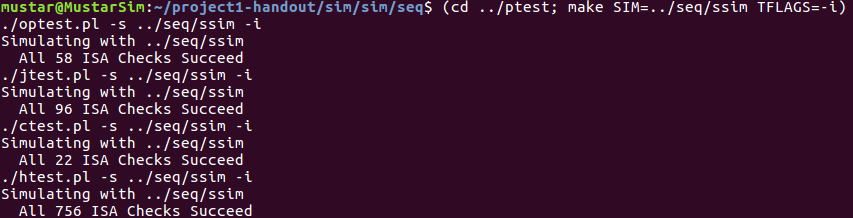
\includegraphics[width=\textwidth]{iaddl test}
	\caption{Regression test(\texttt{iaddl})}
	\end{figure}
\subsection{Part C}

\subsubsection{Analysis}

In this lab, the task should be divided into two parts: hardware optimization and software optimization. And within these evaluation methods, we could not do much hardware optimizations like adding instructions other than \texttt{iaddl} and \texttt{leave}. So the main difficulties lie in the software optimization part.

By adding \texttt{iaddl} and \texttt{leave} instructions we may reduce the average CPE from 16.44 to 12.96, which still above the minimum request.

We found that the main performance limiting factors are two: the data hazard caused by unreasonable register sequence, and the stalling caused by jumping and branching.

For the first problem, we introduced two solutions, \textbf{switching the execution order} (which can be seen in around the \texttt{N1} and \texttt{Twom} label), and use \textbf{multiplexing}, a natural optimization by loop unrolling, to delay register read/write after memory fetching (which can be seen in around the \texttt{Fourm} label).

For the second problem, we used a technique called \textbf{loop unrolling}, to reduce the time. Unlike the traditional way, dividing the loop into quotient and remainder, we divide the loop into a $2^4$ main loop and $2^3$, $2^2$, $2^1$, $2^0$ sub-loops. The latter four will only execute no more than once and can be checked using \texttt{andl}, which could save more instructions.

After these optimization the average CPE would be reduced to 9.45, which is acceptable in this evaluation.


\subsubsection{Code}

\begin{itemize}
	\item \textbf{ncopy.ys}
\begin{lstlisting}
# You can modify this portion
  # Loop header
  xorl %eax,%eax          # count = 0;
  andl %edx,%edx          # len <= 0?
  jle Done                # if so, goto Done:
  
  irmovl $1, %esi
  andl %edx, %esi         # even number?
  je Twom                 # if not so, goto Twom:
  
  mrmovl (%ebx), %esi     # read val from src...
  iaddl $4, %ebx          # src++ fill the bubble
  rmmovl %esi, (%ecx)     # ...and store it to dst
  andl %esi, %esi         # val <= 0?
  jle N1                  # if so, goto N1:
  iaddl $1, %eax          # count++
N1: iaddl $4, %ecx        # dst++
  iaddl $-1, %edx         # len-- <= 0?
  jle Done                # if so, goto Done:
Twom: irmovl $2, %esi 
  andl %edx, %esi         # 1 mod 2 number?
  je Fourm                # if not, goto Fourm:
  
  mrmovl (%ebx), %esi     # read val from src...
  iaddl $8, %ebx          # src+=2 fill the bubble
  rmmovl %esi, (%ecx)
  andl %esi, %esi         # val <= 0?
  jle N2                  # if so, goto N2:
  iaddl $1, %eax          # count++
N2:
  mrmovl -4(%ebx), %esi   # read val from src...
  iaddl $8, %ecx          # dst+=2 fill the bubble
  rmmovl %esi, -4(%ecx)   # ...and store it to dst
  andl %esi, %esi         # val <= 0?
  jle N3                  # if so, goto N3:
  iaddl $1, %eax          # count++
N3: iaddl $-2, %edx       # len-=2 <= 0?
  jle Done                # if so, goto Done:

Fourm: irmovl $4, %esi    # === 4 mod 8 part
  andl %edx, %esi
  je Eightm               # skip if 0 mod 8

  mrmovl (%ebx), %esi     # read val from src...
  mrmovl 4(%ebx), %edi
  rmmovl %esi, (%ecx)     # ...and store it to dst
  rmmovl %edi, 4(%ecx)    # This prevents hazard
  andl %esi, %esi         # val <= 0?       
  jle N4                  # if so, goto N4:
  iaddl $1, %eax          # count++
N4: andl %edi, %edi       # val <= 0?
  jle N5                  # if so, goto N5:
  iaddl $1, %eax          # count++
N5:
  mrmovl 8(%ebx), %esi    # read val from src...
  mrmovl 12(%ebx), %edi
  rmmovl %esi, 8(%ecx)    # ...and store it to dst
  rmmovl %edi, 12(%ecx)  
  andl %esi, %esi         # val <= 0?  
  jle N6                  # if so, goto N6:
  iaddl $1, %eax          # count++
N6: andl %edi, %edi       # val <= 0?  
  jle N7                  # if so, goto N7:
  iaddl $1, %eax          # count++
N7: iaddl $16, %ebx       # src+=4
  iaddl $16, %ecx         # dst+=4
  iaddl $-4, %edx         # len-=4 <= 0?
  jle Done                # if so, goto Done:

Eightm: irmovl $8, %esi   # === 8 mod 16
  andl %edx, %esi
  je Hexm

  mrmovl (%ebx), %esi     # read val from src...
  mrmovl 4(%ebx), %edi
  rmmovl %esi, (%ecx)     # ...and store it to dst
  rmmovl %edi, 4(%ecx)  
  andl %esi, %esi         # val <= 0?  
  jle N8                  # if so, goto N8:
  iaddl $1, %eax          # count++
N8: andl %edi, %edi       # val <= 0?  
  jle N9                  # if so, goto N9:
  iaddl $1, %eax          # count++
N9:
  mrmovl 8(%ebx), %esi    # read val from src...
  mrmovl 12(%ebx), %edi
  rmmovl %esi, 8(%ecx)    # ...and store it to dst
  rmmovl %edi, 12(%ecx)  
  andl %esi, %esi         # val <= 0?  
  jle N10                 # if so, goto N10:
  iaddl $1, %eax          # count++
N10: andl %edi, %edi      # val <= 0?  
  jle N11                 # if so, goto N11:
  iaddl $1, %eax          # count++
N11:
  mrmovl 16(%ebx), %esi   # read val from src...
  mrmovl 20(%ebx), %edi
  rmmovl %esi, 16(%ecx)   # ...and store it to dst  
  rmmovl %edi, 20(%ecx)  
  andl %esi, %esi         # val <= 0?  
  jle N12                 # if so, goto N12:
  iaddl $1, %eax          # count++
N12: andl %edi, %edi      # val <= 0?  
  jle N13                 # if so, goto N13:
  iaddl $1, %eax          # count++
N13:
  mrmovl 24(%ebx), %esi   # read val from src...
  mrmovl 28(%ebx), %edi
  rmmovl %esi, 24(%ecx)   # ...and store it to dst  
  rmmovl %edi, 28(%ecx)  
  andl %esi, %esi         # val <= 0?  
  jle N14                 # if so, goto N14:
  iaddl $1, %eax          # count++
N14: andl %edi, %edi      # val <= 0?  
  jle N15                 # if so, goto N15:
  iaddl $1, %eax          # count++
N15: iaddl $32, %ebx      # src+=8
  iaddl $32, %ecx         # dst+=8
  iaddl $-8, %edx         # len-=8 <= 0?
  jle Done                # if so, goto Done:

Hexm: # The main loop
  mrmovl (%ebx), %esi     # read val from src...
  mrmovl 4(%ebx), %edi
  rmmovl %esi, (%ecx)     # ...and store it to dst
  rmmovl %edi, 4(%ecx)  
  andl %esi, %esi         # val <= 0?  
  jle N16                 # if so, goto N16:
  iaddl $1, %eax          # count++
N16: andl %edi, %edi      # val <= 0?  
  jle N17                 # if so, goto N17:
  iaddl $1, %eax          # count++
N17:
  mrmovl 8(%ebx), %esi    # read val from src...
  mrmovl 12(%ebx), %edi
  rmmovl %esi, 8(%ecx)    # ...and store it to dst
  rmmovl %edi, 12(%ecx)  
  andl %esi, %esi         # val <= 0?  
  jle N18                 # if so, goto N18:
  iaddl $1, %eax          # count++
N18: andl %edi, %edi      # val <= 0?  
  jle N19                 # if so, goto N19:
  iaddl $1, %eax          # count++
N19:
  mrmovl 16(%ebx), %esi   # read val from src...
  mrmovl 20(%ebx), %edi
  rmmovl %esi, 16(%ecx)   # ...and store it to dst  
  rmmovl %edi, 20(%ecx)  
  andl %esi, %esi         # val <= 0?  
  jle N20                 # if so, goto N20:
  iaddl $1, %eax          # count++
N20: andl %edi, %edi      # val <= 0?  
  jle N21                 # if so, goto N21:
  iaddl $1, %eax          # count++
N21:
  mrmovl 24(%ebx), %esi   # read val from src...
  mrmovl 28(%ebx), %edi
  rmmovl %esi, 24(%ecx)   # ...and store it to dst    
  rmmovl %edi, 28(%ecx)  
  andl %esi, %esi         # val <= 0?  
  jle N22                 # if so, goto N22:
  iaddl $1, %eax          # count++
N22: andl %edi, %edi      # val <= 0?  
  jle N23                 # if so, goto N23:
  iaddl $1, %eax          # count++
N23:
  mrmovl 32(%ebx), %esi   # read val from src...
  mrmovl 36(%ebx), %edi
  rmmovl %esi, 32(%ecx)   # ...and store it to dst    
  rmmovl %edi, 36(%ecx)  
  andl %esi, %esi         # val <= 0?  
  jle N24                 # if so, goto N24:
  iaddl $1, %eax          # count++
N24: andl %edi, %edi      # val <= 0?  
  jle N25                 # if so, goto N25:
  iaddl $1, %eax          # count++
N25:
  mrmovl 40(%ebx), %esi   # read val from src...
  mrmovl 44(%ebx), %edi
  rmmovl %esi, 40(%ecx)   # ...and store it to dst    
  rmmovl %edi, 44(%ecx)  
  andl %esi, %esi         # val <= 0?  
  jle N26                 # if so, goto N26:
  iaddl $1, %eax          # count++
N26: andl %edi, %edi      # val <= 0?  
  jle N27                 # if so, goto N27:
  iaddl $1, %eax          # count++
N27:
  mrmovl 48(%ebx), %esi   # read val from src...
  mrmovl 52(%ebx), %edi
  rmmovl %esi, 48(%ecx)   # ...and store it to dst    
  rmmovl %edi, 52(%ecx)  
  andl %esi, %esi         # val <= 0?  
  jle N28                 # if so, goto N28:
  iaddl $1, %eax          # count++
N28: andl %edi, %edi      # val <= 0?  
  jle N29                 # if so, goto N29:
  iaddl $1, %eax          # count++
N29:
  mrmovl 56(%ebx), %esi   # read val from src...
  mrmovl 60(%ebx), %edi
  rmmovl %esi, 56(%ecx)   # ...and store it to dst    
  rmmovl %edi, 60(%ecx)  
  andl %esi, %esi         # val <= 0?  
  jle N30                 # if so, goto N30:
  iaddl $1, %eax          # count++
N30: andl %edi, %edi      # val <= 0?  
  jle N31                 # if so, goto N31:
  iaddl $1, %eax          # count++
N31: iaddl $64, %ebx      # src+=16
  iaddl $64, %ecx         # dst+=16
  iaddl $-16, %edx        # len-=8 > 0?
  jg Hexm                 # if so, goto Hexm.
##################################################################
# Do not modify the following section of code
# Function epilogue.
Done:
  popl %edi       # Restore callee-save registers
  popl %ebx
  popl %esi
  leave
  ret
		\end{lstlisting}
	\item \textbf{pipe-full.hcl}

\begin{lstlisting}
# Is instruction valid?
bool instr_valid = f_icode in
	{ INOP, IHALT, IRRMOVL, IIRMOVL, IRMMOVL, IMRMOVL,
	  IOPL, IJXX, ICALL, IRET, IPUSHL, IPOPL, IIADDL, ILEAVE };
...
# Does fetched instruction require a regid byte?
bool need_regids =
	f_icode in { IRRMOVL, IOPL, IPUSHL, IPOPL, 
		     IIRMOVL, IRMMOVL, IMRMOVL, IIADDL };

# Does fetched instruction require a constant word?
bool need_valC =
	f_icode in { IIRMOVL, IRMMOVL, IMRMOVL, IJXX, ICALL, IIADDL };
...
## What register should be used as the A source?
int d_srcA = [
	D_icode in { IRRMOVL, IRMMOVL, IOPL, IPUSHL  } : D_rA;
	D_icode in { IPOPL, IRET } : RESP;
	D_icode in { ILEAVE } : REBP;
	1 : RNONE; # Don't need register
];

## What register should be used as the B source?
int d_srcB = [
	D_icode in { IOPL, IRMMOVL, IMRMOVL, IIADDL } : D_rB;
	D_icode in { IPUSHL, IPOPL, ICALL, IRET, ILEAVE } : RESP;
	1 : RNONE;  # Don't need register
];

## What register should be used as the E destination?
int d_dstE = [
	D_icode in { IRRMOVL, IIRMOVL, IOPL, IIADDL } : D_rB;
	D_icode in { IPUSHL, IPOPL, ICALL, IRET, ILEAVE } : RESP;
	1 : RNONE;  # Don't write any register
];

## What register should be used as the M destination?
int d_dstM = [
	D_icode in { IMRMOVL, IPOPL } : D_rA;
	D_icode in { ILEAVE } : REBP;
	1 : RNONE;  # Don't write any register
];
...
## Select input A to ALU
int aluA = [
	E_icode in { IRRMOVL, IOPL, ILEAVE } : E_valA;
	E_icode in { IIRMOVL, IRMMOVL, IMRMOVL, IIADDL } : E_valC;
	E_icode in { ICALL, IPUSHL } : -4;
	E_icode in { IRET, IPOPL } : 4;
	# Other instructions don't need ALU
];

## Select input B to ALU
int aluB = [
	E_icode in { IRMMOVL, IMRMOVL, IOPL, ICALL, 
		     IPUSHL, IRET, IPOPL, IIADDL } : E_valB;
	E_icode in { IRRMOVL, IIRMOVL } : 0;
	E_icode in { ILEAVE } : 4;
	# Other instructions don't need ALU
];
...
## Should the condition codes be updated?
bool set_cc = E_icode in { IOPL, IIADDL } &&
  # State changes only during normal operation
  !m_stat in { SADR, SINS, SHLT } && !W_stat in { SADR, SINS, SHLT };
...
## Select memory address
int mem_addr = [
	M_icode in { IRMMOVL, IPUSHL, ICALL, IMRMOVL } : M_valE;
	M_icode in { IPOPL, IRET, ILEAVE } : M_valA;
	# Other instructions don't need address
];

## Set read control signal
bool mem_read = M_icode in { IMRMOVL, IPOPL, IRET, ILEAVE };
\end{lstlisting}
\end{itemize}

\subsubsection{Evaluation}

The correctness is shown in the figure below. The original output is quite long, so formatting tools (\texttt{column} from util-linux package) is used.

\begin{figure} [H]
        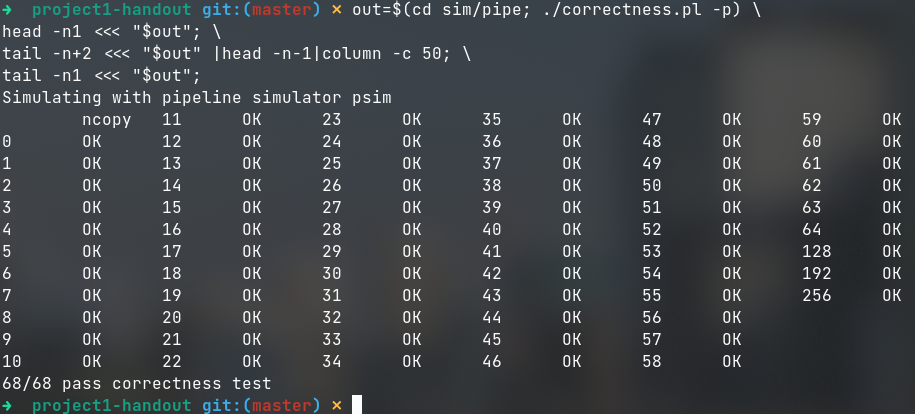
\includegraphics[width=\textwidth]{fig-correctness.png}
        \caption{Correctness (Used format tools to shrink)}
\end{figure}

The performance and benchmark result is shown in the figure below. The original output is quite long, so formatting tools (\texttt{column} from util-linux package) is used.

\begin{figure} [H]
        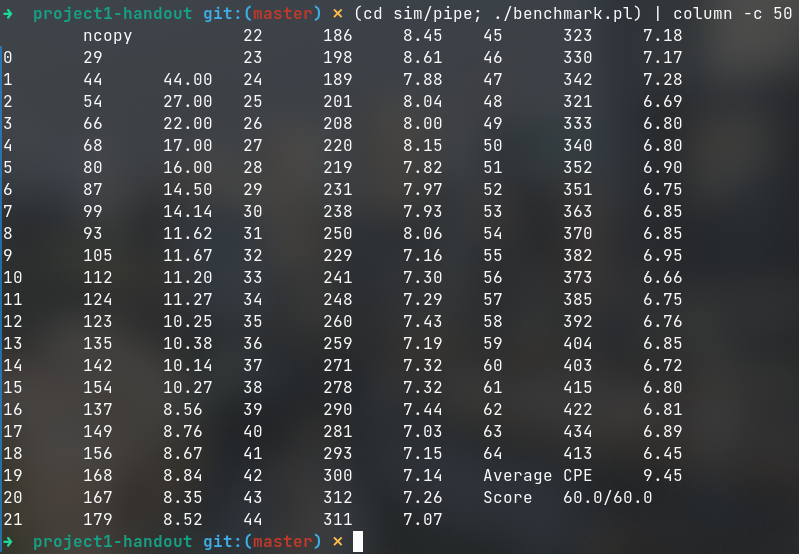
\includegraphics[width=\textwidth]{fig-benchmark.png}
        \caption{Benchmark (Used format tools to shrink)}
\end{figure}

\section{Conclusion}

\subsection{Problems}

\begin{itemize}
	\item \textbf{Part A}
	
		The main obstacle for this part is a quite detailed problem, how to use stack pointers and implement function recursions smartly. Although we have learned a lot about assembly language and read many classic codes, it is still very hard for us to write assembly programs correctly by ourselves. How to arrange the order of pulling elements from stack and implement the function recursion to prevent from cover the values of register by mistake have troubled us a lot. However, by debugging patiently and summarizing from experience, we gradually get the knack. It is of great importance to get fully understand of function of every stack pointer and let them perform as it own function.
		
	\item \textbf{Part B}
	
		Adjusting to the syntax of \texttt{HCL} is the only obstacle of this part. Since we are complete freshmen to \texttt{HCL}, at first it seems that we have no way to start. However, after days of searching and learning, we have gradually adjusted to this new language. And fortunately, it does not need us to fully master it. Moreover, the comments in file also helps a lot. Finally we successfully complete this part.
	\item \textbf{Part C}
	
		After finishing Part A and Part B, we are more familiar with assembly language and the syntax of \texttt{HCL}. So the main obstacles which limit the performance are data hazard caused by unreasonable register sequence and the stalling caused by jumping and branching. We explored for a long time and tried several ways. Ultimately, we switch the execution order and use multiplexing to solve the first problem. As for the second, we use a technique called loop unrolling to reduce time.
\end{itemize}

\subsection{Achievements}
First, we are more familiar computer architecture and linux operations after writing assembly programs and extending the SEQ processor to support a new instruction with our own hands. What's more, the process of optimizing in Part C also brought us a keen appreciation for the interactions between the software and the hardware, which affect the performance of programs. And these experience could never be replaced by textbooks and oral teaching.

Second, it is reletively exicted to achieve an average CPE less than 10.0 after careful design of logic and implementation. Moreover, considerable optimizations were made after achieving full score of Part C, which also brought us a sense of achievement and taught us to persistently improve.

Third, we have also gained a lot of experience of partner coooeration from this project. Since a member of our group, Wanting Li has never used git before, it is her first experience to collaborate with partner online to complete a project, which is precious and pragmatic. And this also made us put a lot of effort into the readability of codes and leave sufficient comments, which cultivated a good habit of programming. What's more, the process of completing this project also make both of us to reap the valuable sense of accomplishment and have a deeper understanding of cooperation.

Finally, we would like to specially thank Miss Shen and TAs for their kind and patient support. And we are also grateful to Shanghai Jiao Tong University and School of Electronic Information and Electrical Engineering to provide such a valuable and interesting course.


%----------------------------------------------------------------------------------------


\end{document}
